%
% slopes.tex
%
% (c) 2018 Prof Dr Andreas Müller, Hochschule Rapperswil
%
\documentclass[tikz]{standalone}
\usepackage{times}
\usepackage{amsmath}
\usepackage{txfonts}
\usepackage[utf8]{inputenc}
\usepackage{graphics}
\usetikzlibrary{arrows,intersections}
\begin{document}

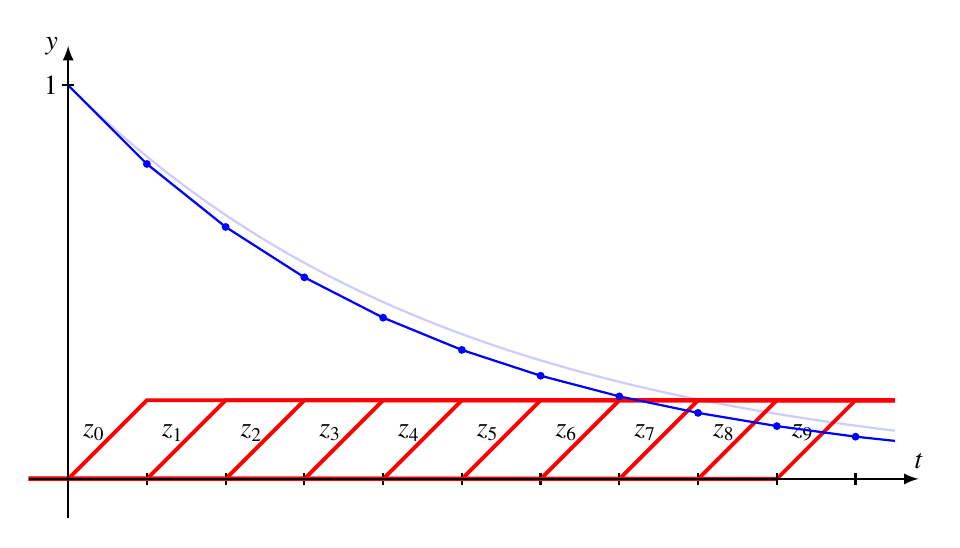
\begin{tikzpicture}[>=latex,thick]

\draw[color=blue!20] plot[domain=0:10.5,samples=100] ({\x},{5*exp(-\x / 5)});

\def\yfunktion#1{
	\draw[color=red,line width=1.4pt] (-0.5,0)--({#1},0)--({#1+1},1)--(10.5,1);
	\node at ({#1+0.6},0.35) [above left] {$z_{#1}$};
	\draw ({#1},-0.08)--({#1},0.08);
}

\begin{scope}

\clip (-0.5,-0.5) rectangle (10.5,1.5);
\foreach \x in {0,1,...,9}{
	\yfunktion{\x}
}
\end{scope}

\def\ynull{1}
\def\yeins{0.8}

\begin{scope}
\clip (-0.5,-0.5) rectangle (10.5,5.5);
\foreach \x in {0,1,...,10}{
	\draw[color=blue] ({\x},{5*\ynull})--({\x+1},{5*\yeins});
	\fill[color=blue] ({\x+1},{5*\yeins}) circle[radius=0.05];
	\xdef\ynull{\yeins}
	\pgfmathparse{\ynull * 0.8}
	\xdef\yeins{\pgfmathresult}
	%\draw[color=blue,line width=0.1pt] ({\x+1},{5*\ynull})--({\x+1},1);
}
\end{scope}

\draw[->] (-0.5,0)--(10.8,0) coordinate[label=$t$];
\draw[->] (0,-0.5)--(0,5.5) coordinate[label={left:$y$}];

\draw (10,-0.08)--(10,0.08);

\draw (-0.08,5)--(0.08,5);
\node at (0,5) [left] {$1$};

\end{tikzpicture}

\end{document}
